
\documentclass[modern]{aastex63}
\usepackage{graphicx}
\usepackage{subfigure}
\usepackage{multirow}
\usepackage{comment}
\usepackage{natbib}
\usepackage{hyperref}
\usepackage{mathtools}
\usepackage{longtable}
\usepackage{mathrsfs}
\usepackage{fontenc}
\usepackage{color}
\usepackage{url}
\usepackage{hyperref}
\usepackage{gensymb}
\usepackage{pifont}



\begin{document}
\title{Final Project Reports}
\author{Yu Qiu}
\affiliation{Kavli Institute for Astronomy and Astrophysic \\
Peking University \\
Beijing 100871, China}
\author{Yuxuan Pang}
\affiliation{Kavli Institute for Astronomy and Astrophysic \\
Peking University \\
Beijing 100871, China}
\author{Zhiwei Pan}
\affiliation{Kavli Institute for Astronomy and Astrophysic \\
Peking University \\
Beijing 100871, China}
\email{1901110222.pku.edu.cn}
\email{1901110223.pku.edu.cn}
\email{1901110222.pku.edu.cn}

\begin{abstract}
In this project, we study the methods of open cluster membership selection and discuss the appliable conditions for simple method. We also use the photomerty and astrometry information from Gaia DR2 to estimate the age of individual cluster from literature by CMD isochrone fitting. At last, we study the evolution peroperties of open cluster.


\end{abstract}

\keywords{open cluster --- astrometry --- CMD --- evolution}


\section{Introduction}\label{sec:intro}
An Open Cluster(OC) is a group of up to a few thousand stars that were formed from the same giant molecular cloud and have roughly the same age. The study of OCs stellar population, formation and evolution has a great contribution to modern astrophysics. From their star formation process, the assembly and evolution of the Milky Way disc can be studied(\cite{2016A&A...591A..37J},\cite{2016A&A...588A.120C}); from their spatial distribution and motion, the gravitational potential and the perturbations of Milky Way disc could be better understand; from their age distribution, the Galactic structure can be traced(\cite{2014MNRAS.444..290B}). OCs are also popular tracers to follow the metallicity gradient of the Milky Way(\cite{2017MNRAS.470.4363C})and its evolution through time(\cite{2016A&A...585A.150N}). 

In addition to useful tracers of the Milky way, OCs are interesting targets in their own right. The most important characteristic of the OCs is that they are loosely bound by mutual gravitational attraction and will gradually lose their stellar content. Generally, their evolution can be split into three phases: (i) the first lasts for $\sim$ 3 Myr, during which the cluster in embedded in its progenitor molecular cloud and stars are still forming; (ii) then the clusters experience the expulsion of the residual star-forming gas; and finally, (iii) the long term evolutionary phase dominated by both internal and external dynamical processes.
	
\emph{Gaia} second data release in 2018(\cite{2018A&A...616A..12G}) has opened a new era in cluster science. Before \emph{Gaia}, \cite{2013A&A...558A..53K} listed about 3000 OCs candidates, then \cite{2018A&A...618A..93C} use the membership assignment code
UPMASK (Unsupervised Photometric Membership Assignment in Stellar Clusters, \cite{2014A&A...561A..57K}) determine 1229 OCs' members. \cite{2019A&A...623A.108B} applied an automated Bayesian tool, BASE-9, to fit stellar isochrones and finally gives 269 OCs' age. Our project aims to reproduce a general process for analyzing star clusters from data, which divide into three parts. 
In the first part, we try to give a method to distinguish a star cluster from the field stars. The previous method mainly including two kinds of method, first is divided stars into different magnitude band then select a typical radius for each band by eye[citation], and second method is using a PCA program to determine the candidates first(\cite{2018A&A...618A..93C}). Both the method also use the restriction of proper-motion and location of the star. 
In the second part,  

Since their population may cover a wide range of age and some physcical properties, we can investigate the relation between the mass, radius or velocity dispersion and age to trace the evolution of these properties and find out how the clusters dissipate and lose stellar mass and maybe some other interesting things.

Our summary is organised as follows: in Section \ref{selection}, we will talk about selection. In Section \ref{age}, we will talk abput age. In Section \ref{evolution}, we will talk about evolution. In Section \ref{con}, we will make a summary.

\bigskip
\bigskip
\section{Cluster Membership selection}\label{selection}






\bigskip
\bigskip
\section{age determination}\label{age}




\bigskip
\bigskip
\section{evolution of open clusters}\label{evolution}
In this section, we will talk about the dynamical properties and evolution of the open clusters, which mainly focuses on the dissipation of the cluster. Firstly, we will introduce the determination of several parameters including the velocity dispersion $\sigma_v$, dynamical evolution parameter $\tau$, that is useful to describe the dynamical properties and evolution. Then, we will present some results and analysis.

\subsection{Cluster Parameters} 
With the help of Gaia DR2, Cantat-Gaudin et al. (2018) has established the list of 1229 clusters which have at least five stars with a membership probability greater than 50\%. Also he compiled the catalogue of all the candidate stars of 1229 clusters. We use their catalogue to get the additional kinematic and dynamical parameters.
%————————————————————————————————————————————————————————————————————————————————————————————————
% figure
\begin{figure}[t]
\centering
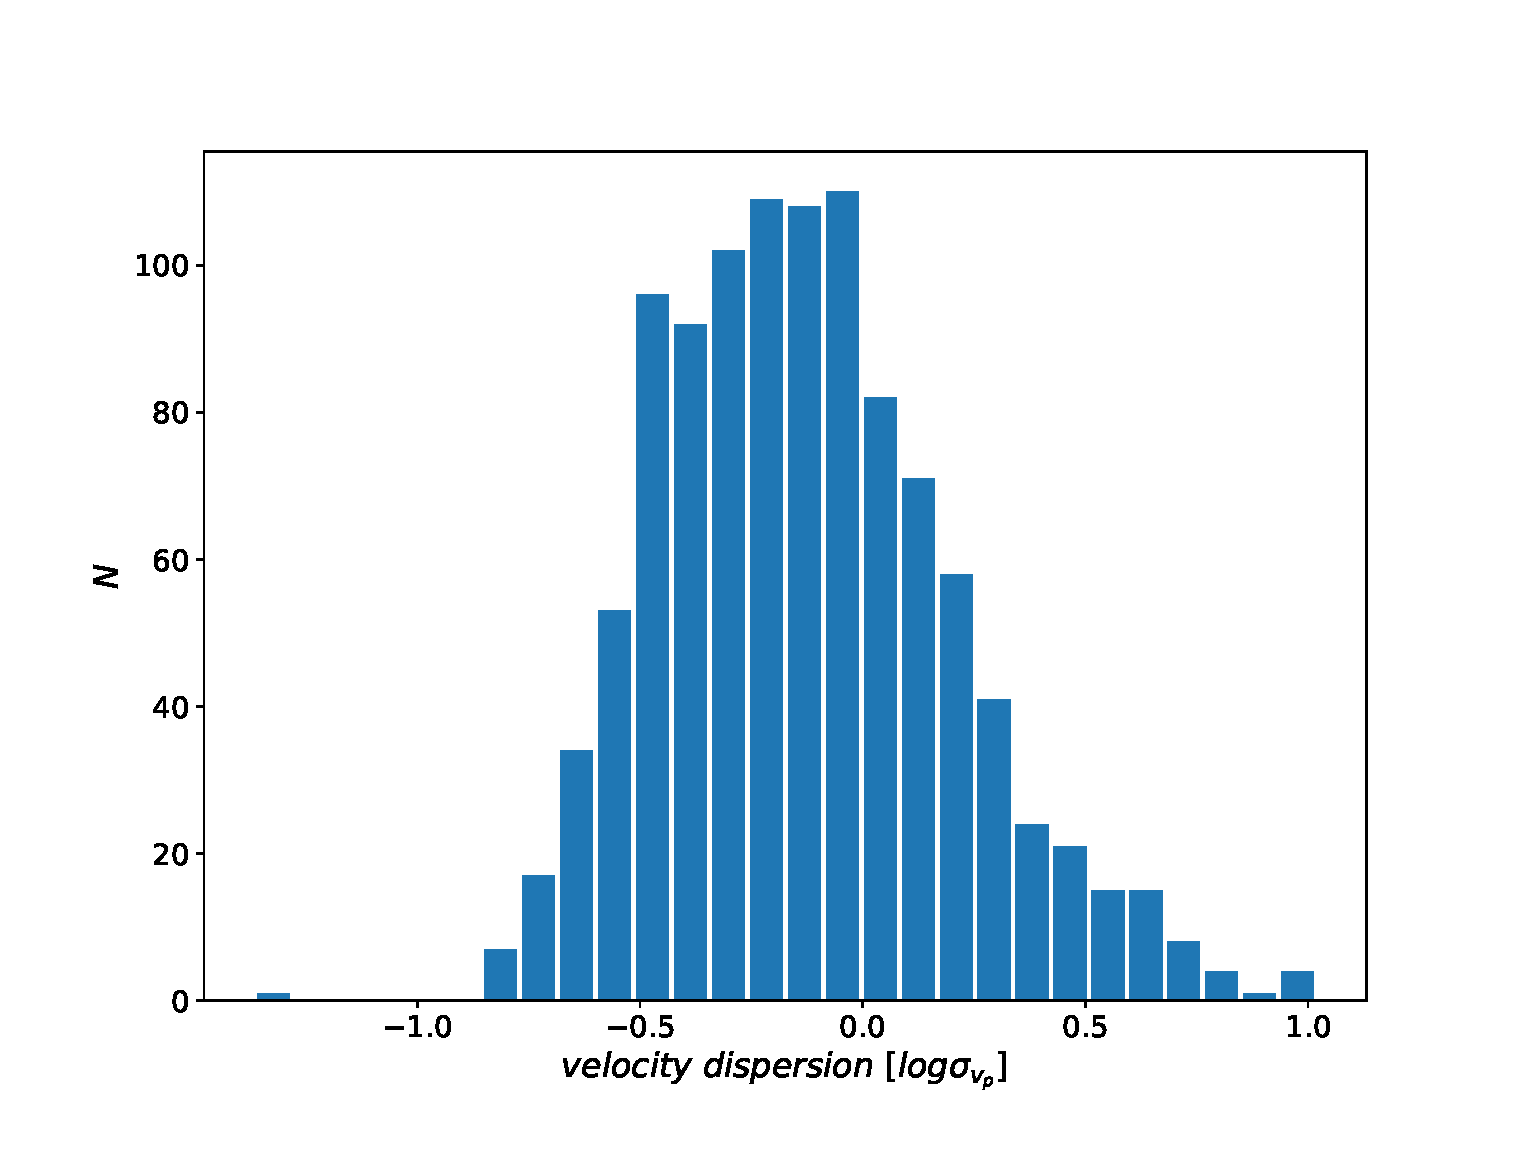
\includegraphics[width=0.49\linewidth]{6.eps}
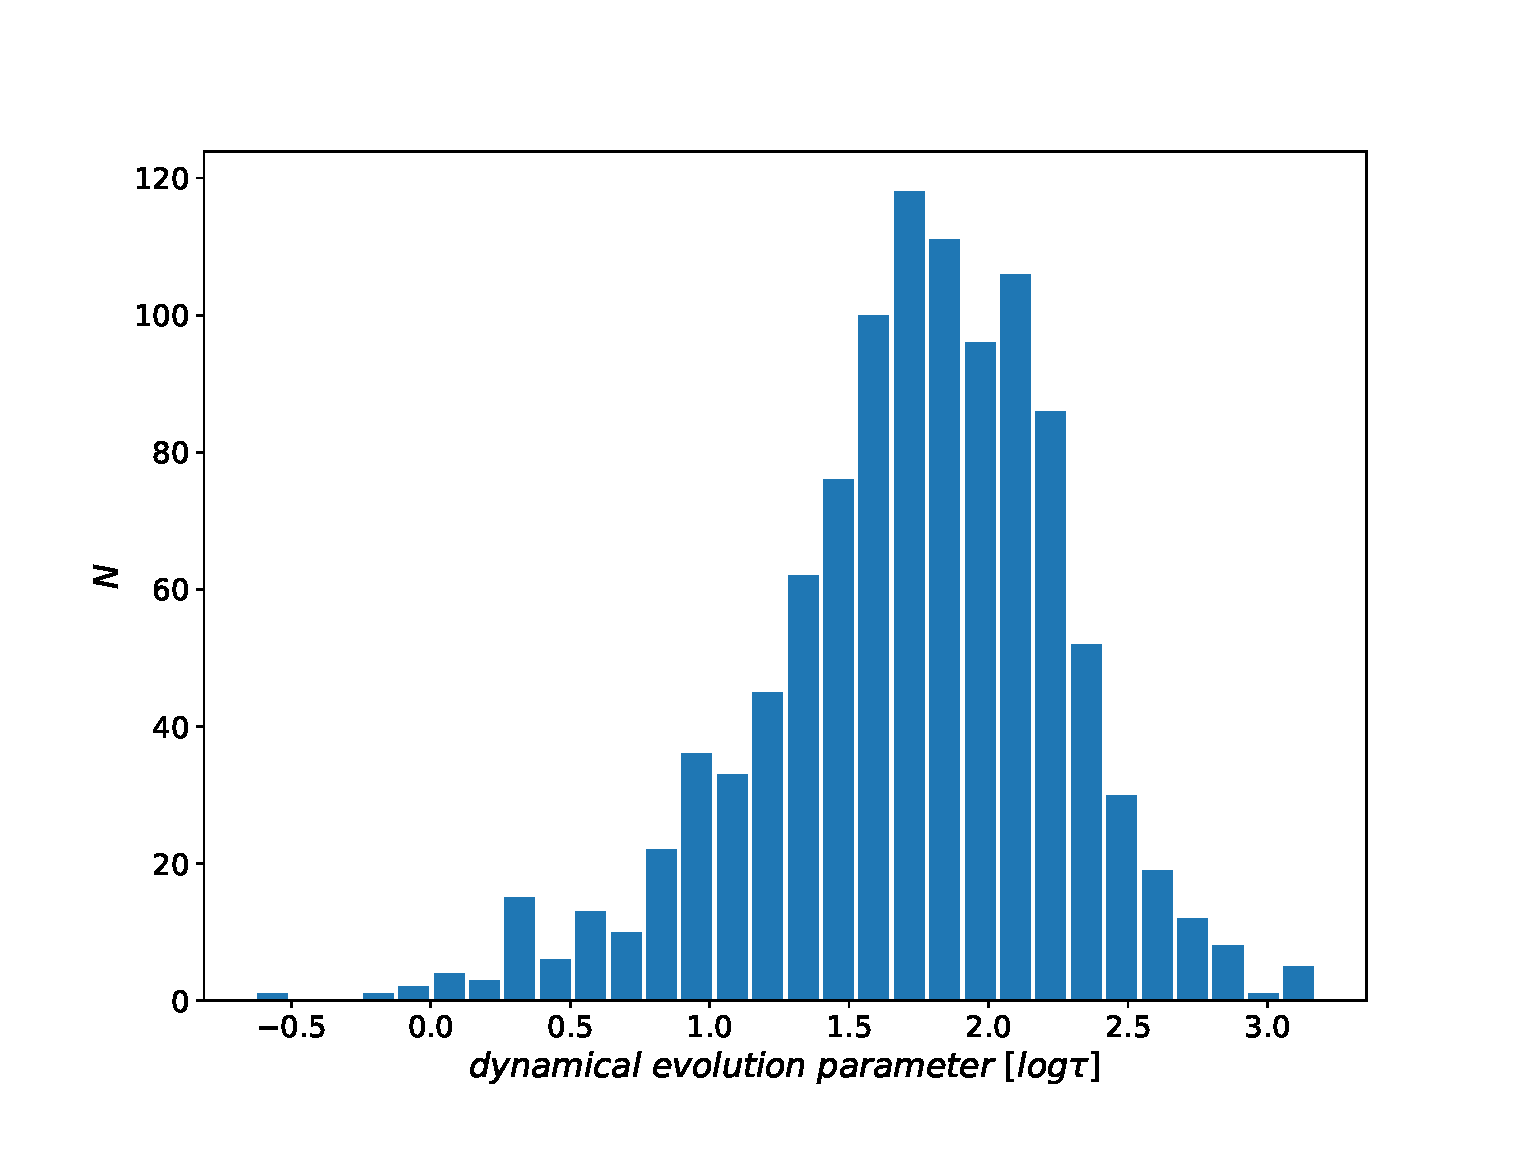
\includegraphics[width=0.49\linewidth]{7.eps}
%\includegraphics[width=7.5cm]{fig1c.eps}
\caption{Distribution of the velocity dispersion and dynamical evolution parameter.}
\label{1}
\end{figure}
%figure
%———————————————————————————————————————————————————————————————————————————————————————————————
As stars' proper motion in right ascension $\mu_{\alpha_*}$ and declination $\mu_{\delta}$ and the parralax $\varpi$ have been provided and the mean proper motion $\bar{\mu}_{\alpha_*}$, $\bar{\mu}_{\delta}$ of each cluster has also been computed, we can calculate the proper motion of each star relative to its cluster centroid through $\mu_{\alpha_*}^{\prime}=\mu_{\alpha_*}-\bar{\mu}_{\alpha_*}$ and $\mu_{\delta}^{\prime}=\mu_{\delta}-\bar{\mu}_{\delta}$. Then we follow a procedure analogous to that of Cantat-Gaudin et al. (2018), an iterative 2$\sigma$ clipping exclusion routine, to process the data of $\mu_{\alpha_*}^{\prime}$ and $\mu_{\delta}^{\prime}$ to get the proper motion velocity dispersion which is shown in Figure \ref{1}. Such a procedure is meant to exclude the dispersion caused by the background noise and determine the true velocity dispersion $\sigma_{v_p}$. While the proper motion velocity dispersion is 2-dimensional, it can roughly satisfy our needs to analyze the dynamical properties of the open cluster. Actually 3D velocity dispersion $\sigma_v$ can be estimated by $\sigma_v=\sqrt{3/2}\sigma_{v_p}$ assuming that velocity components of stars relative to each object centre are isotropically distributed.

Althougth in Secion \ref{age}, we already obtained the age of each cluster, it hardly helps us understand the evolution of the cluster because different clusters have different evoution timescale. For an open cluster, internal interaction is considered to be important in shaping the structure and promoting the dynamical evolution. Stellar encounters are one of the important interactions whose characteristic time is called relaxation time. Following Spitzer \& Hart (1971), the relaxation time for a stellar system is
\begin{equation*}
T_R=\frac{8.9\times10^5\sqrt{N}\times R^{1.5}_h}{\sqrt{m}\times \log{0.4N}}
\end{equation*}
where $N$ is the number of the cluster members, $R_h$ is the radius containing half of the cluster mass in parsecs, and $m$ is the average mass of the cluster in solor unit. The related parameters can all be obtained from the catalogue(Cantat-Gaudin et al. 2018) and Section \ref{age}. Then with the age $t$ of each cluster, we can define the dynamical evolution parameter $\tau$ as $\tau=t/T_R$ which is appropriate to stand for the evolutionary phase of different clusters.
The result is shown in Figure \ref{1}.

Other parameters like the distance to the galactic plane $Z$ and G-band maginitude can be easily get from the catalogue.


\subsection{Results and Discussion}
%————————————————————————————————————————————————————————————————————————————————————————————————
% figure
\begin{figure}[t]
\centering
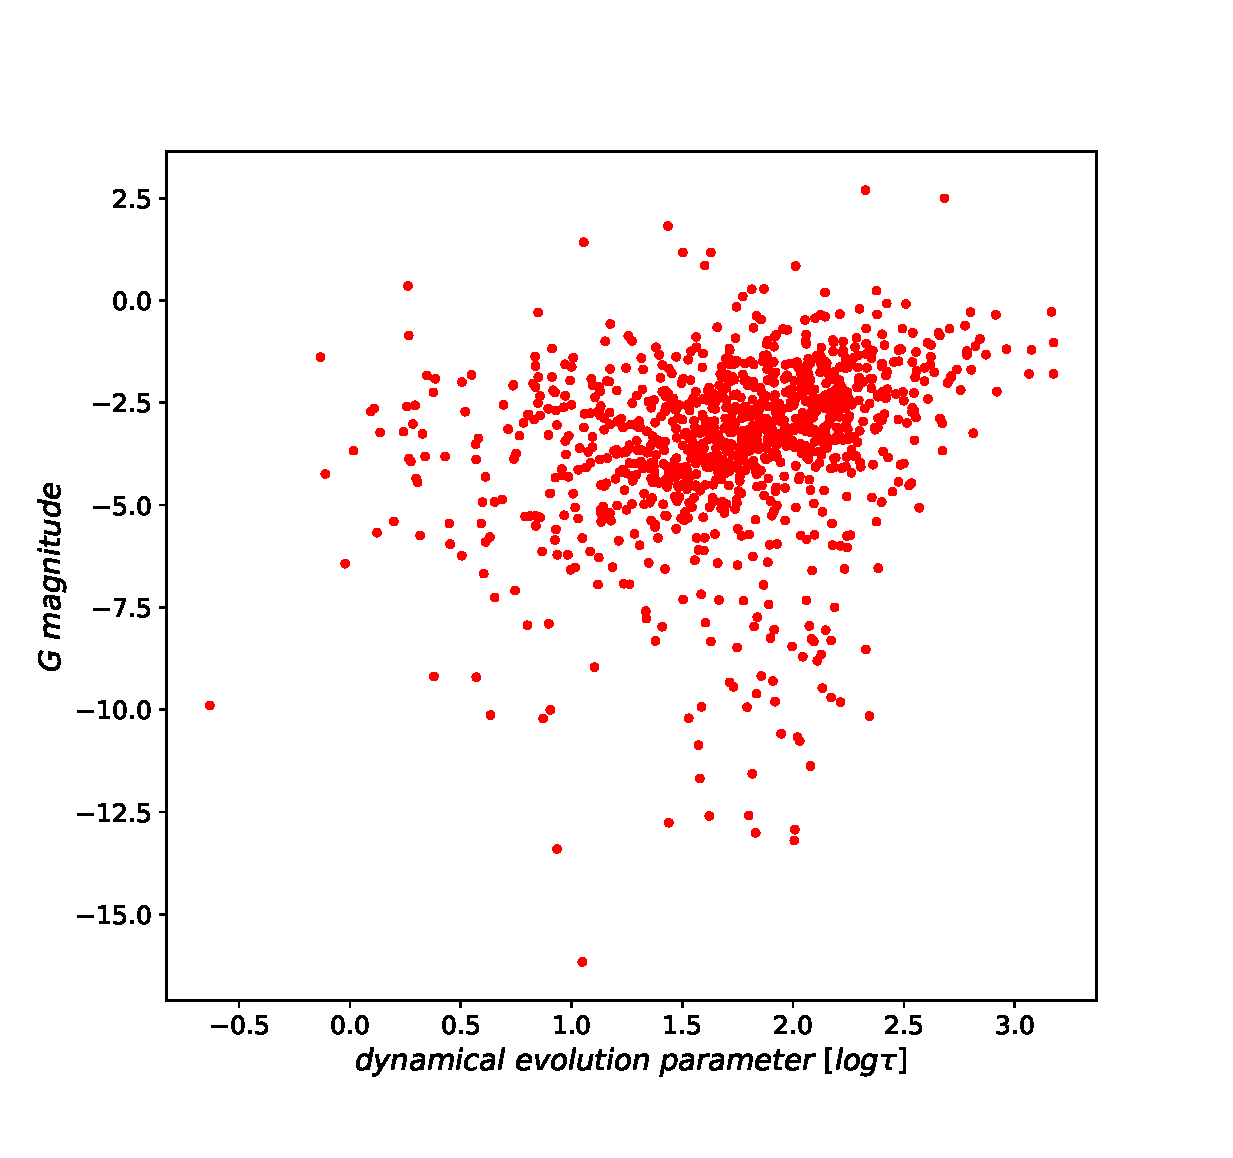
\includegraphics[width=0.49\linewidth]{1.eps}
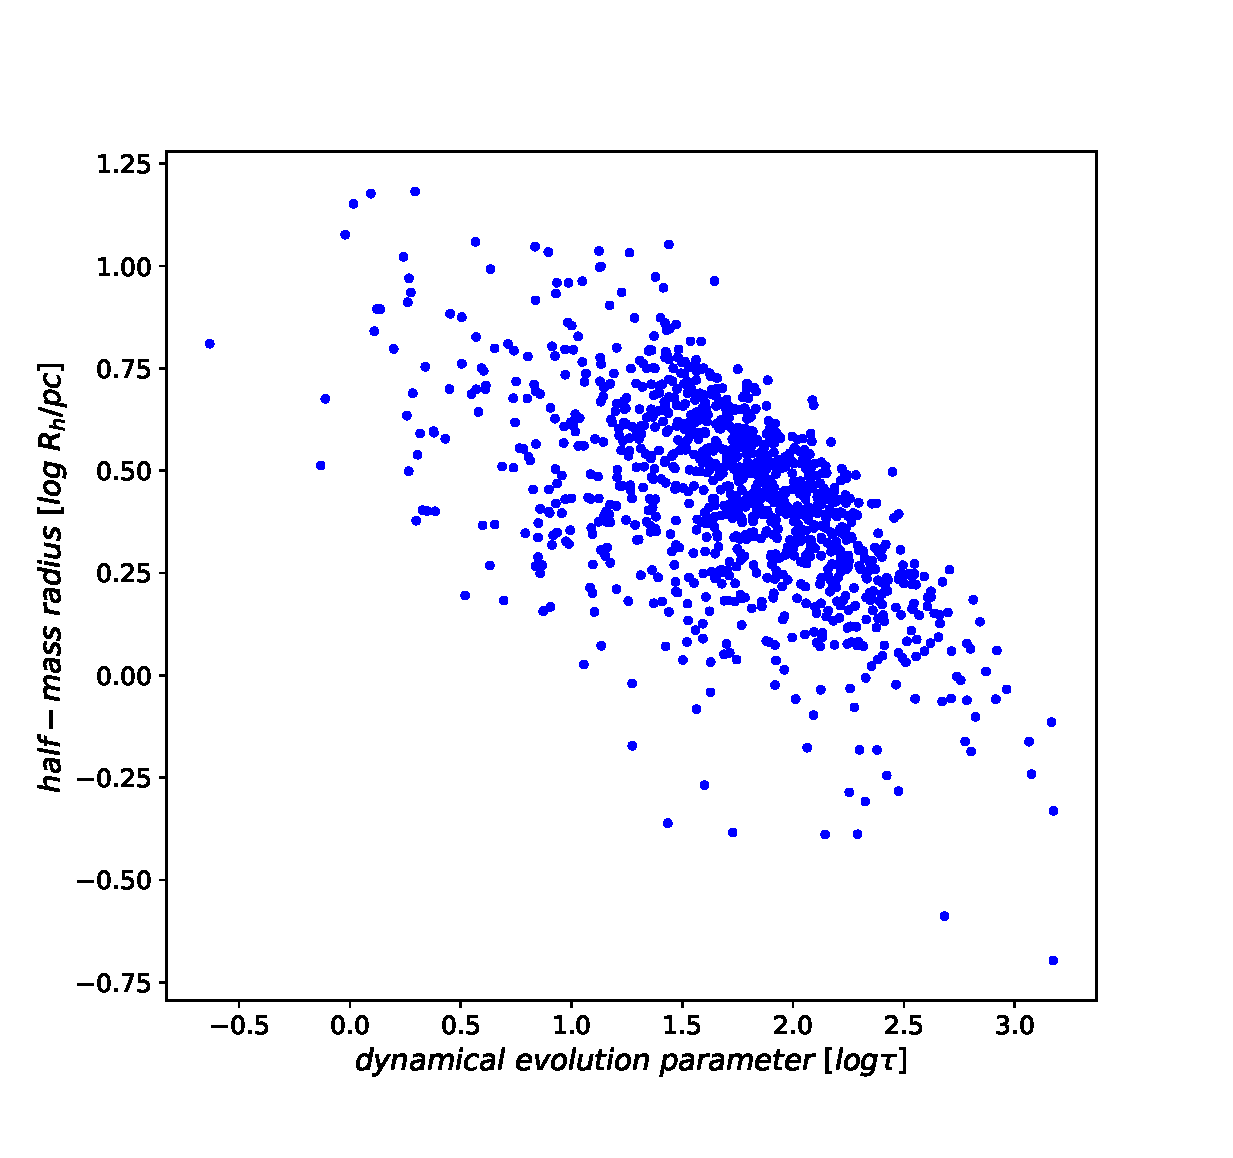
\includegraphics[width=0.49\linewidth]{2.eps}
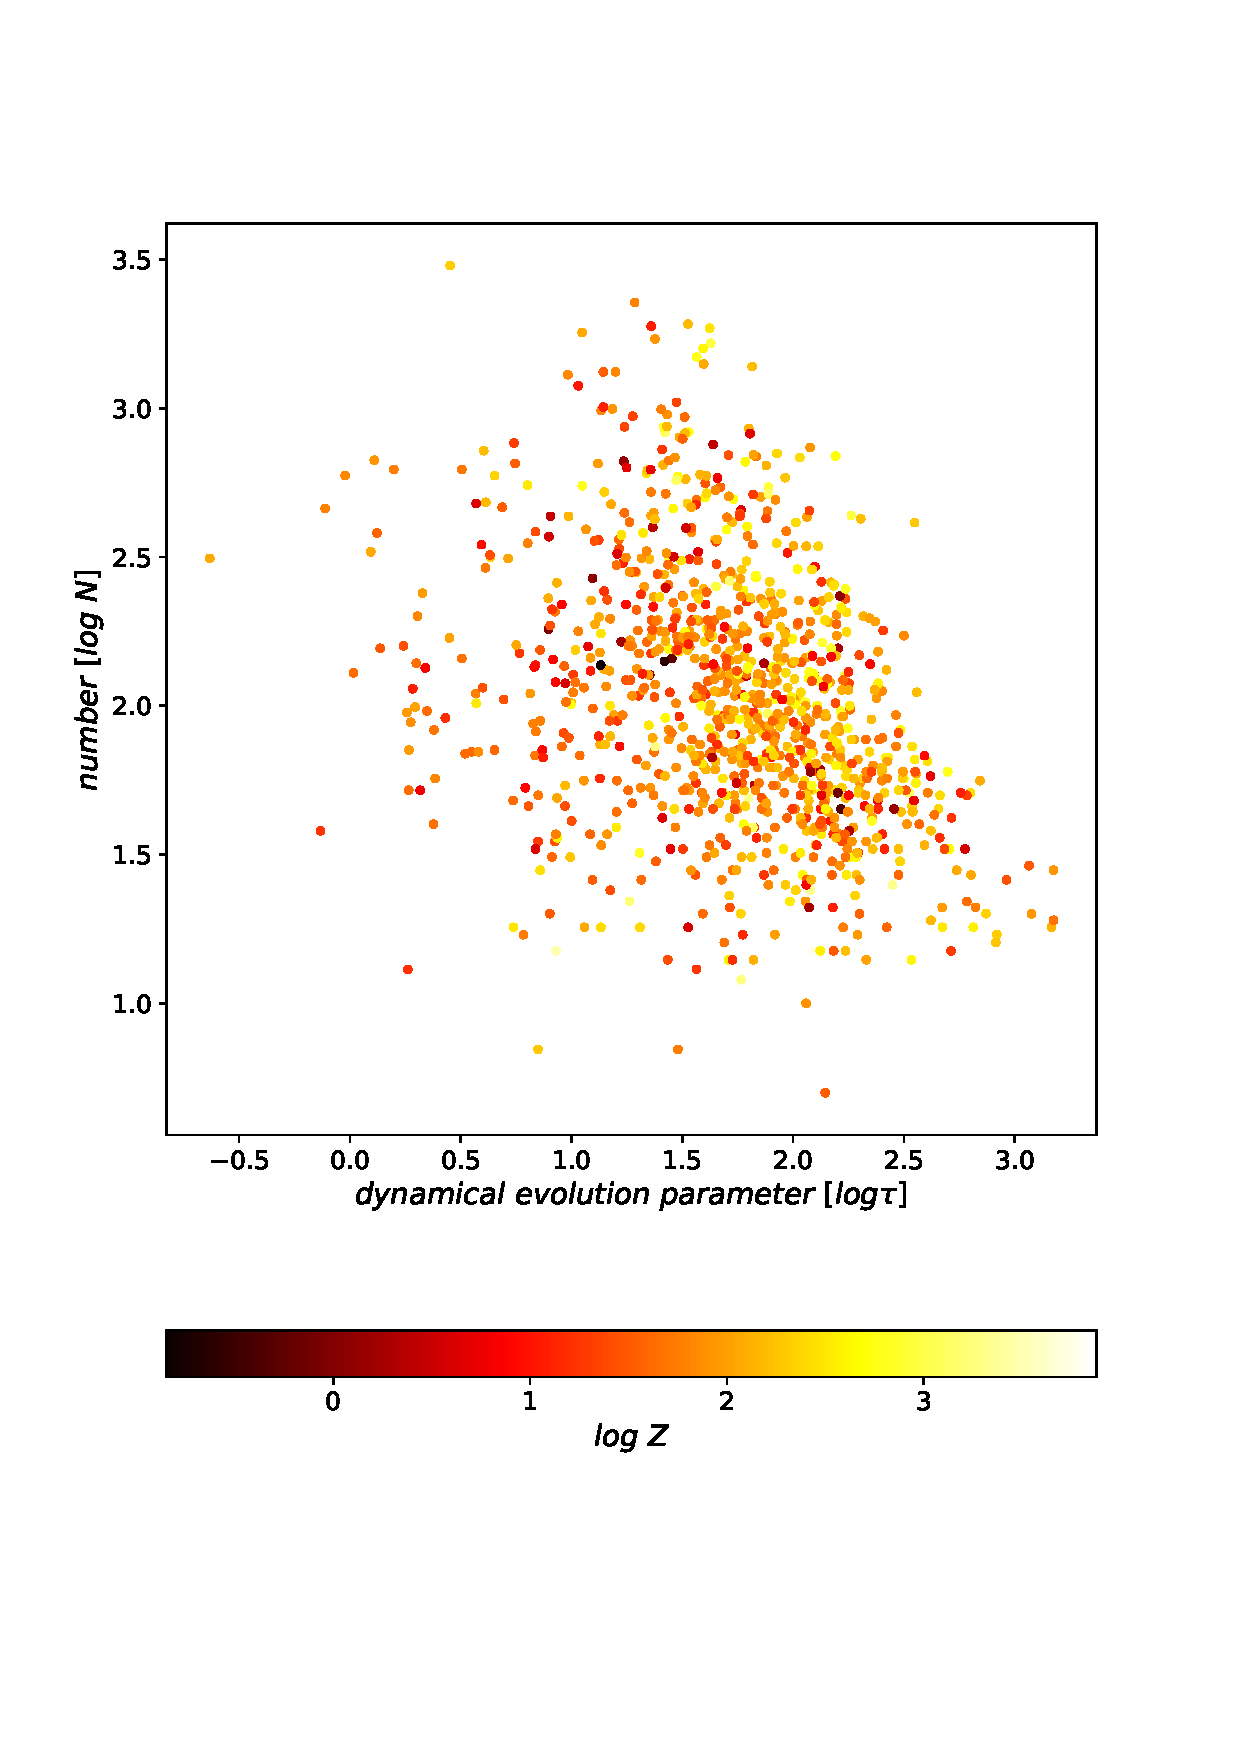
\includegraphics[width=0.49\linewidth]{3.eps}
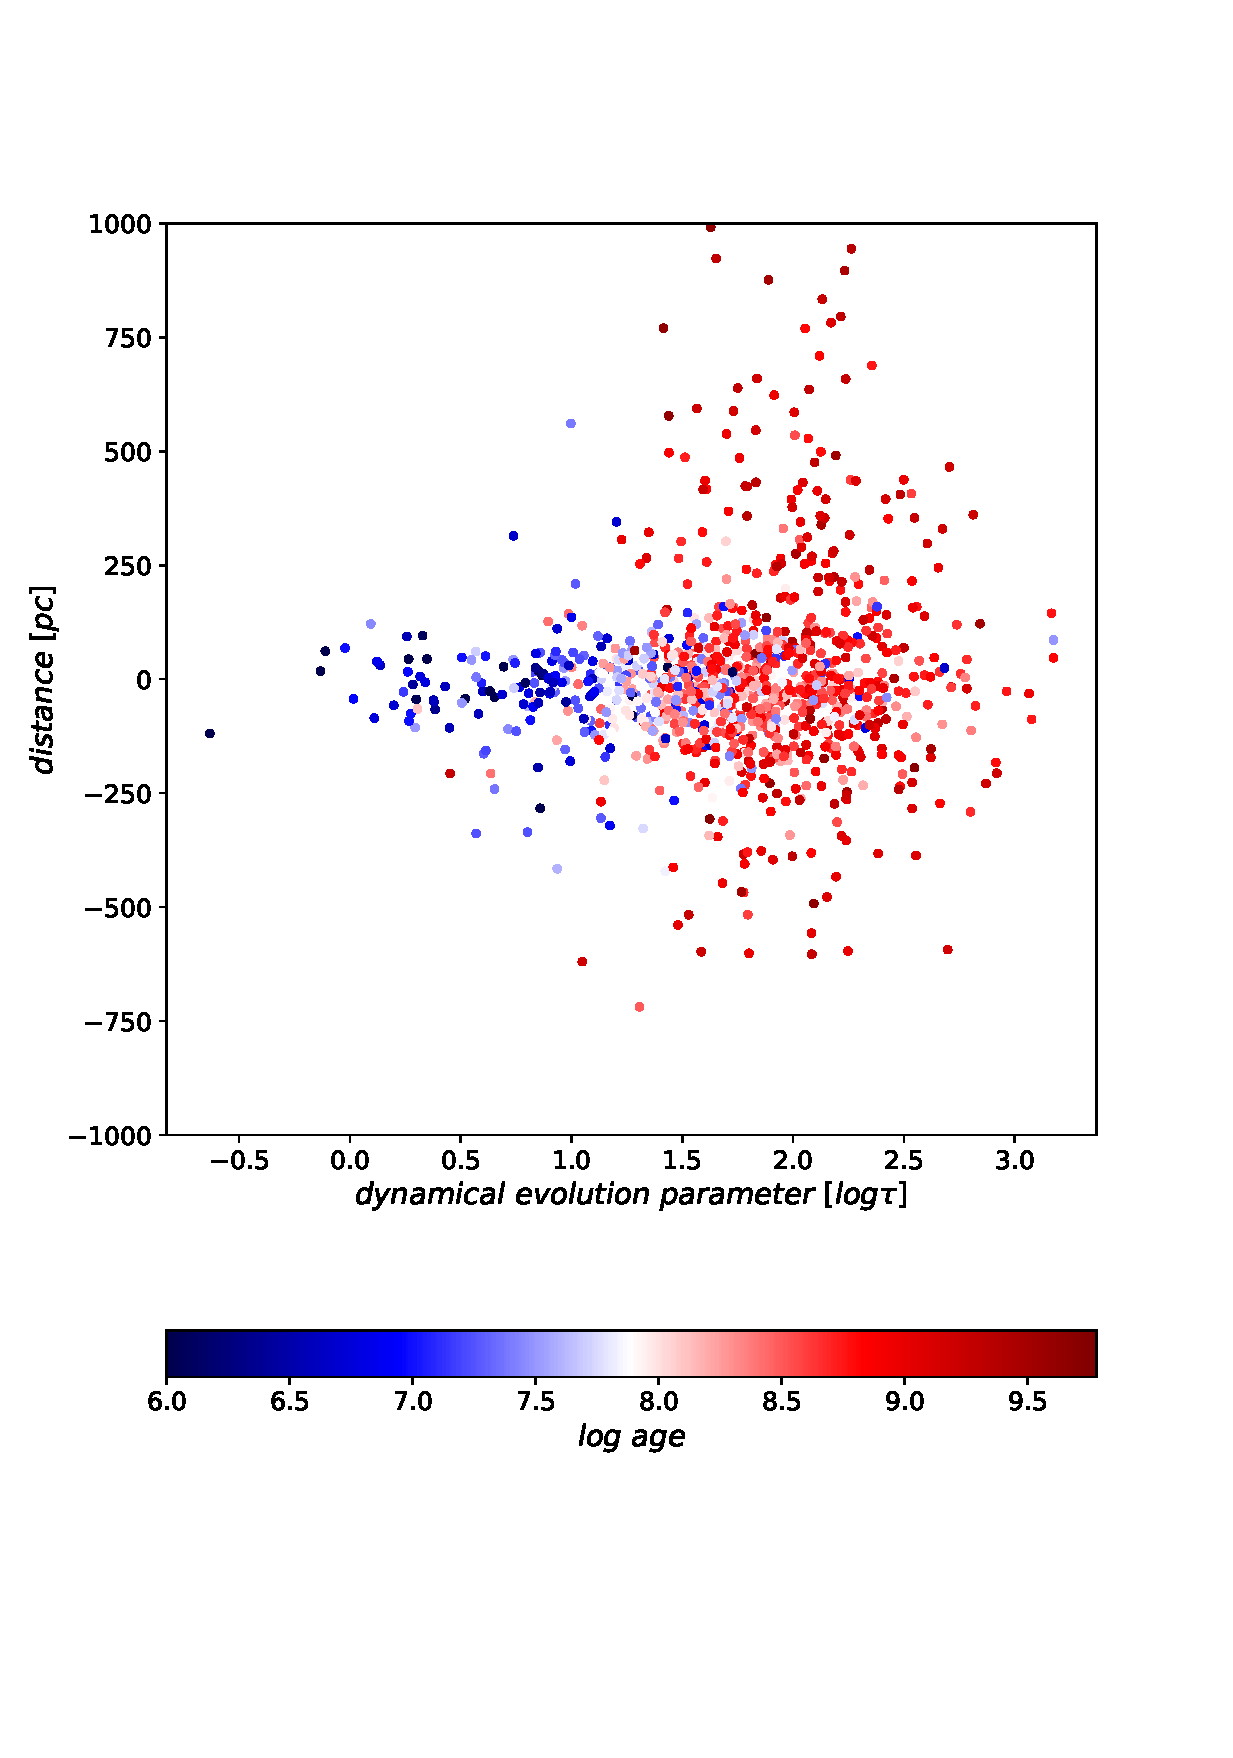
\includegraphics[width=0.49\linewidth]{4.eps}
%\includegraphics[width=7.5cm]{fig1c.eps}
\caption{different properties versus the dynamical evolution parameter of the open cluster. Each dot in the four plots stands for one cluster.}
\label{2}
\end{figure}
%figure
%———————————————————————————————————————————————————————————————————————————————————————————————

With most parameters of clusters obtained, we can just plot the different properties versus the dynamical evolution parameter to investigate the evolution of the cluster. 
Figure \ref{2} shows four properties of the cluster: G-band magnitude, size, number of members, the distance to the galactic plane.

From the two plots in the upper panel, we can roughly see the change during the evolution. The G-band magnitude becomes larger as the dynamical evolution parameter increases which implies that the luminosity may gradually decrease and it is a natural result as the stars continue to evolve. The right plot present a more apparent trend that the half-mass radius decreases during the evolution. This is mainly because of the dissipation of the open cluster which is also reflected from the left plot in the bottom panel. We can clearly see the number of members of the cluster decreases from up to $10^3$ to $10$. We input the distance to the galactic plane in the color and it seems that the decreasing trend also holds for the similar color which implies that the stellar encounters as a form of internal interaction play an important role in mass loss of the cluster in the long-term evolutionary phase($t\gtrsim100\mathrm{Myr}$). And in the right panel we show the distance to the galactic plane will have large scatter in the later evolution. And these clusters that are away from the plane also overlaps those very old clusters which indicates that the high galactic latitude region is also a livable place for the very old cluster because of avoiding some external interaction like disk shocking that can disrupt the cluster.

%————————————————————————————————————————————————————————————————————————————————————————————————
% figure
\begin{figure}[t]
\centering
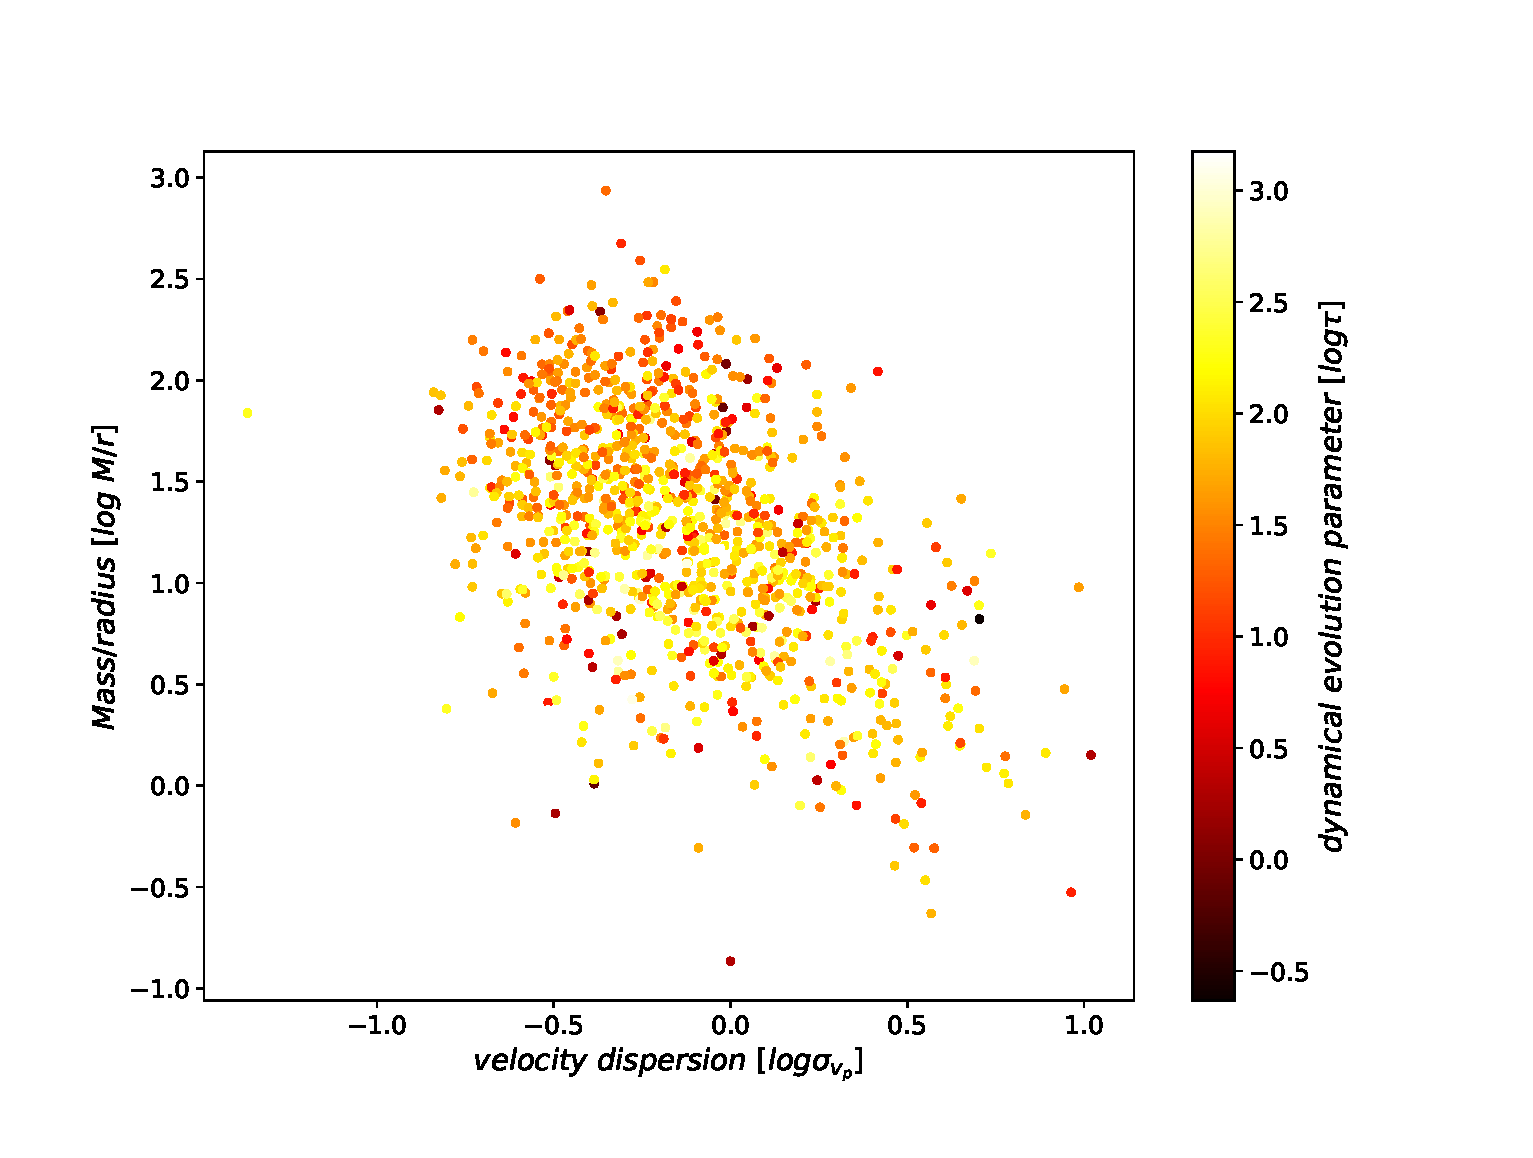
\includegraphics[width=1\linewidth]{5.eps}

%\includegraphics[width=7.5cm]{fig1c.eps}
\caption{$\log M/r$ versus $\log \sigma_{v_p}$.}
\label{3}
\end{figure}
%figure
%———————————————————————————————————————————————————————————————————————————————————————————————
We also try to investigate the dynamical state of the cluster so we plot the $\log M/r$ versus $\log \sigma_{v_p}$, which is shown in Figure \ref{3}. But the relation seems to disobey the virial theorem which is not affected by different evolutionary phase. We consider it maybe caused by the error in the proper motion detection and the mass underestimation during the CMD fit. Nevertheless, it does not affect our previous analysis and argument.

\bigskip
\bigskip
\section{conclusions}\label{con}
In this project, we study the methods of open cluster membership selection and discuss the appliable conditions for simple method. We also use the photomerty and astrometry information from Gaia DR2 to estimate the age of individual cluster from literature by CMD isochrone fitting. At last, we study the evolution peroperties of open cluster.

We investigate the evolution of the open cluster using the dynamical evolution parameter as a tracer. It is demostrated that the luminosity, size and number of members will decrease during the evolution. We reveal the role of internal and external interaction in the evolution of open clusters and argue that the stellar encounters can significantly cause the mass loss and the external interaction like disk shock will affect the cluster migration and distribution.


\acknowledgments
We sincerely thank to Xiaoting Fu's generous help and advice.

\newpage
\bibliography{colloquim}{}
\bibliographystyle{aasjournal1}






\end{document}

% End of file `sample63.tex'.